\section{The Components of the Jeliot~3 System}
\label{sec:The_Components_of_the_Jeliot_3_System}


\subsection{User Interface}
\label{sec:User_Interface}

The design of the user inteface is a crucial aspect in the tool for novice computer user.
We used the user interface design from Jeliot 2000 as it was found usable and simple for novices \citep{Levy2003}.
We have just added extra menus and short keys to make the lecture use of
the software smoother. Moreover, the line numbering was added to the code editor and view to
make the referencing to the code easier. The user interface of Jeliot~3 and its layout is
illustrated in the Figures~\ref{fig:jeliot3_UI_structure} and \ref{fig:jeliot3_theatre_structure}.

- Picture of the user interface.

\begin{figure}[!htb]
\begin{center}
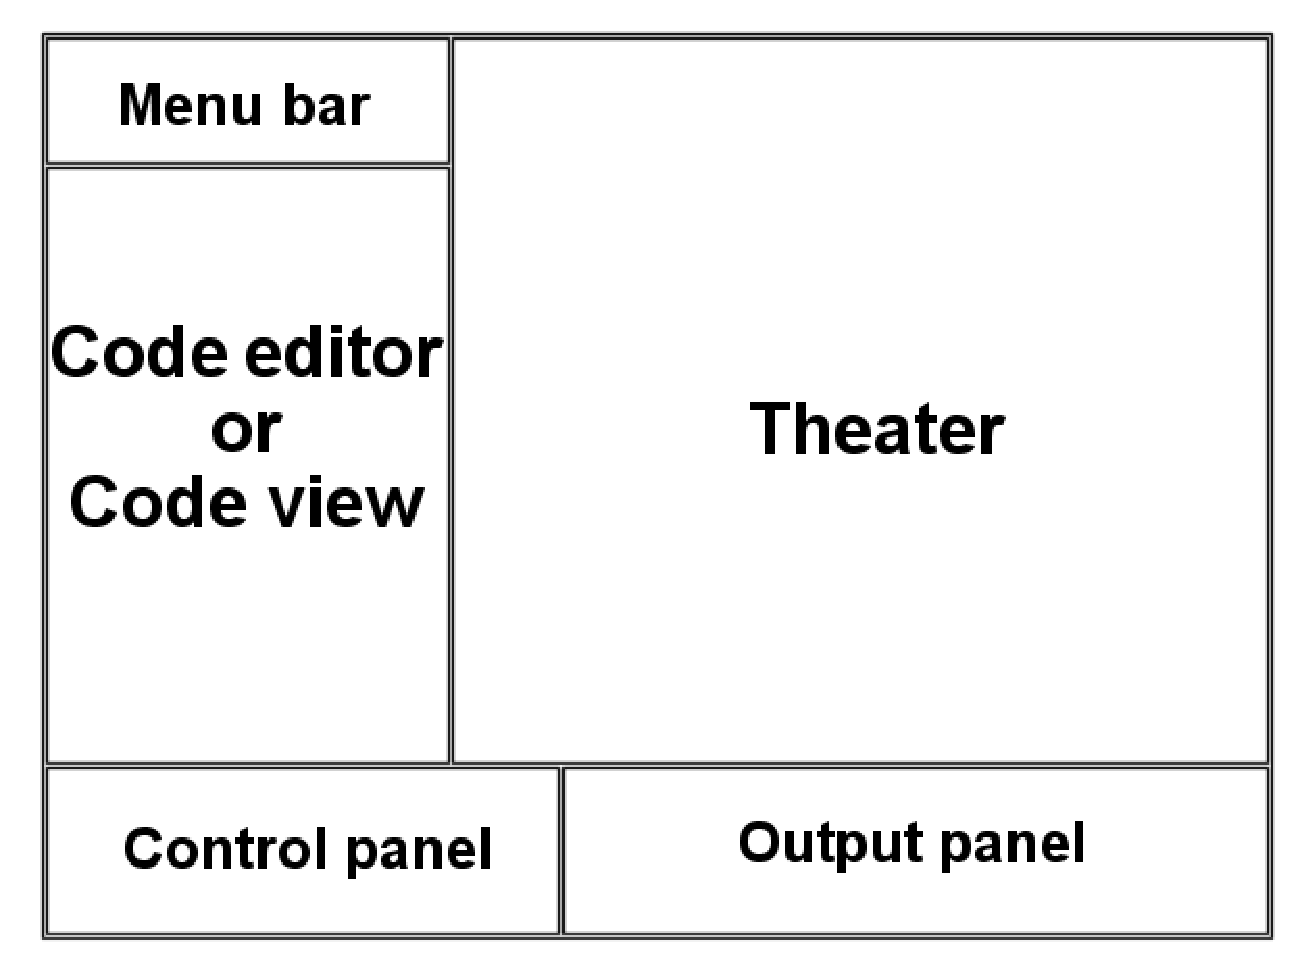
\includegraphics[height=10cm]{jeliot3_UI_structure.eps}
\caption{The structure of user interface in Jeliot~3.}
\label{fig:jeliot3_UI_structure}
\end{center}
\end{figure}


\begin{figure}[!htb]
\begin{center}
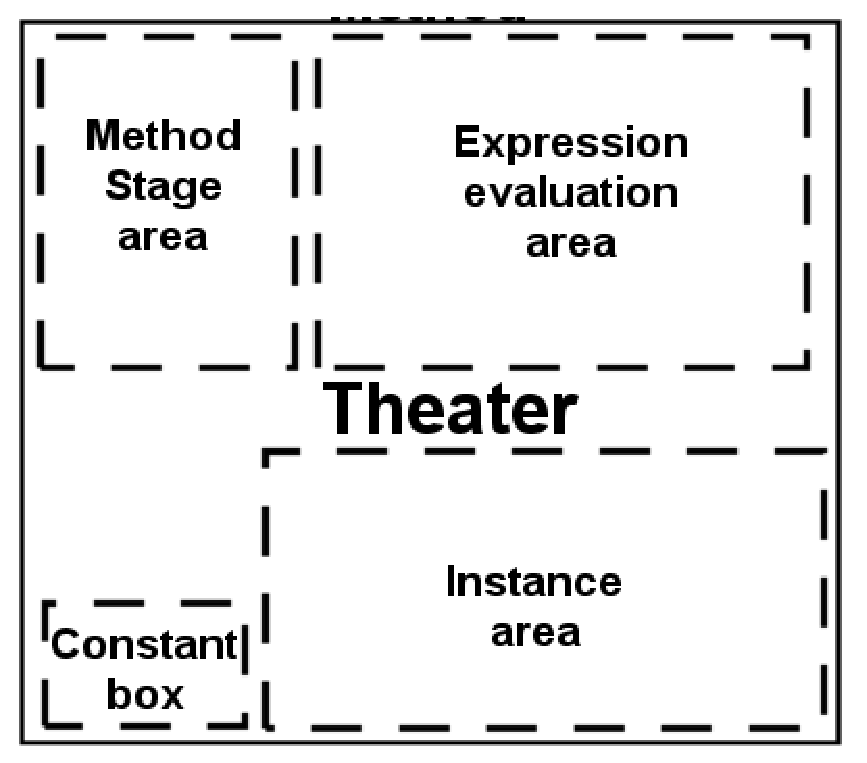
\includegraphics[height=8cm]{jeliot3_theatre_structure.eps}
\caption{The structure of the animation frame (theatre) in Jeliot~3.}
\label{fig:jeliot3_theatre_structure}
\end{center}
\end{figure}

\subsection{DynamicJava}
\label{sec:DynamicJava}

DynamicJava consists of 7 different packages, where only five
of them actually perform the interpretation: \p{classfile}, \p{classinfo},
\p{interpreter}, \p{parser} and \p{tree}. The other two (\p{util} and \p{gui}) are
used to help the debugging of DynamicJava and to provide a nicer
user interface to the interpreter. For example, the \p{displayVisitor},
included in the util package, provides a nice output from the syntax tree.

\begin{itemize}
\item \p{Classfile} contains all the classes for creating general purpose bytecode
classes. The most important class is ClassFile which is the heart
of the class creation process.

\item \p{Classinfo} contains all the classes and interfaces for using reflection
on Java or interpreted classes. This package is used during
the compilation of the classes.

\item \p{Interpreter} contains the classes for interpreting Java language statements.
This is the most important package. It contains the most important
visitors that will be explained later.

\item \p{Parser} provides the classes that compose the default parser for the
language. The parser itself is represented by the class Parser.
The parser is generated by JavaCC 1.0. It creates the nodes of the
tree to be traversed later by the interpreter visitors.

\item \p{Tree} provides classes and interfaces for producing an abstract syntax
tree. This package does not depend of any non standard java package.
\end{itemize}

The created tree consists of nodes, the main data structure used
in DynamicJava. All nodes have common properties, the segment
of source code where that node refers. Subclasses of this node
are defined to address the unique properties of each different
Java (e.g. staments and constructions). For example a node for
any binary expression will also consist of the properties \p{LEFT\_EXRESSION}
and \p{RIGHT\_EXPRESSION}.

Figure \ref{fig:Packages_visitors_and_data_flow_in_DJava} explains the
main relationships between the packages, the visitors and the main data flow.

\begin{figure}[htbp]
\begin{center}
\begin{picture}(400,200)
\put(110,20){\framebox(270,130){\ }}
\put(220,20){\makebox(50,20){\f{Interpreter}}}

\put(0,50){
\put(0,15){\vector(1,0){40}}
\put(0,15){\makebox(40,20){\shortstack{\f{source}\\\f{code}}}}
\put(40,0){\framebox(50,30){\f{Parser}}}
\put(90,15){\vector(1,0){40}}
\put(90,15){\makebox(40,20){\f{tree}}}
\put(130,0){\dashbox{5}(55,30){\shortstack{\f{Name}\\\f{Visitor}}}}
\put(180,15){\vector(1,0){40}}
\put(180,15){\makebox(40,20){\f{tree}}}
\put(220,0){\dashbox{5}(55,30){\shortstack{\f{Type}\\\f{Checker}}}}
\put(270,15){\vector(1,0){40}}
\put(270,5){\makebox(40,20){\shortstack{\f{tree}\\\f{and}\\\f{class}}}}
\put(310,0){\dashbox{5}(55,30){\shortstack{\f{Evaluation}\\\f{Visitor}}}}
\put(360,15){\vector(1,0){40}}
\put(360,15){\makebox(40,20){\f{result}}}
}

\put(240,80){\vector(0,1){20}}\put(250,100){\vector(0,-1){20}}
\put(240,130){\vector(0,1){40}}\put(250,170){\vector(0,-1){40}}
\put(60,80){\vector(0,1){90}}\put(70,170){\vector(0,-1){90}}
\put(270,180){\vector(1,0){40}}\put(310,190){\vector(-1,0){40}}

\put(220,100){\dashbox{5}(55,30){\shortstack{\f{TreeClass-}\\\f{Compiler}}}}

\put(0,170){
\put(40,0){\framebox(50,30){{\f{Tree}}}}
\put(220,0){\framebox(50,30){{\f{ClassInfo}}}}
\put(310,0){\framebox(50,30){{\f{ClassFile}}}}
}

\end{picture}
\caption{Packages, visitors and data flow in DynamicJava}
\label{fig:Packages_visitors_and_data_flow_in_DJava}
\end{center}
\end{figure}

As we can see in the image DynamicJava carries the source code
through three visitors: \p{NameVisitor}, \p{TypeChecker} and, finally, \p{EvaluationVisitor}.
We also see how \p{EvaluationVisitor} will receive a class from \p{TypeChecker},
the reason of this behaviour will be explained in the next paragraphs.

The NameVisitor is a tree visitor that resolves the ambiguity in identifiers in a syntax tree.
As declared, this visitor traverses the tree trying to find out syntactical ambiguities.

The \p{TypeChecker} is a tree visitor that checks the typing rules and loads the
classes, fields and methods.
This \p{TypeChecker} class is not only worried about typing rules.
When visiting a class declaration, it invokes \p{TreeCompiler}, which
compile the class into Java bytecode. However this compiling
process \textit{alters the class} and the formed \textit{bytecode does
not match the original source code} of the class.

The \p{EvaluationVisitor} is a tree visitor that evaluates each node of a syntax tree.
This visitor is the one that performs the evaluation and execution
of the program. It usually starts by invoking the main method
of the compiled class. We can easily observe how it traverses
the syntax tree and modifies DynamicJava structures to store information
and thus we can interfere with its normal interpretation to extract
the information it produces while interpreting the source code.


\subsection{Visualization Engine}
\label{sec:Visualization_Engine}


